% =====================================================================
%  MCMP117 -- Fundamentals of Operating Systems
%  Week 2 Course Notes: Definitions, Goals, Components & OS Structures
%  Compile with XeLaTeX (twice):  xelatex MCMP117_Week2_Notes.tex
%  Needs ./figures/ (if present) and the ../code/ folder.
% =====================================================================
\documentclass[11pt,a4paper]{article}
\newcommand{\weeknum}{2}
% ---------- Page & fonts ---------------------------------------------
\usepackage[a4paper,margin=2.3cm,headheight=15pt]{geometry}
\usepackage{fontspec}
\IfFontExistsTF{Calibri}{\setmainfont{Calibri}}{\setmainfont{Carlito}}
\IfFontExistsTF{Cambria}{\newfontfamily\headfont{Cambria}}{\newfontfamily\headfont{Caladea}}
\IfFontExistsTF{Consolas}{\setmonofont[Scale=0.95]{Consolas}}{\setmonofont[Scale=0.88]{DejaVu Sans Mono}}
\usepackage{amsmath,amssymb}
\usepackage{microtype}
\linespread{1.12}
\setlength{\parskip}{0.55em}
\setlength{\parindent}{0pt}

% ---------- Colours (course design system) ----------------------------
\usepackage{xcolor}
\definecolor{dark}{HTML}{212121}
\definecolor{charcoal}{HTML}{36454F}
\definecolor{slate}{HTML}{50808E}
\definecolor{mint}{HTML}{02C39A}
\definecolor{mintdeep}{HTML}{028090}
\definecolor{light}{HTML}{F2F2F2}
\definecolor{muted}{HTML}{6B7679}

% ---------- Packages ---------------------------------------------------
\usepackage{graphicx}
\usepackage{float}
\usepackage{needspace}
\graphicspath{{figures/}}
\usepackage[font=small,labelfont={bf,color=mintdeep},justification=centering]{caption}
\usepackage{booktabs,longtable,array,tabularx}
\usepackage{enumitem}
\setlist{itemsep=0.25em,topsep=0.3em}
\usepackage{tikz}
\usetikzlibrary{arrows.meta,positioning,calc,shapes.geometric}
\usepackage{pgfplots}
\pgfplotsset{compat=1.17}
\usepackage[most]{tcolorbox}
\usepackage{titlesec}
\usepackage{fancyhdr}
\usepackage{xurl}
\usepackage[colorlinks=true,linkcolor=mintdeep,urlcolor=mintdeep,citecolor=mintdeep]{hyperref}

% ---------- Headings ----------------------------------------------------
\titleformat{\section}{\headfont\Large\bfseries\color{charcoal}}{\color{mint}\thesection}{0.7em}{}
\titleformat{\subsection}{\headfont\large\bfseries\color{charcoal}}{\color{mintdeep}\thesubsection}{0.6em}{}
\titleformat{\subsubsection}{\headfont\normalsize\bfseries\color{mintdeep}}{}{0em}{}
\titlespacing*{\section}{0pt}{1.6em}{0.6em}
\titlespacing*{\subsection}{0pt}{1.2em}{0.4em}

% ---------- Header / footer -----------------------------------------------
\pagestyle{fancy}
\fancyhf{}
\fancyhead[L]{\small\color{muted}MCMP117 --- Fundamentals of Operating Systems}
\fancyhead[R]{\small\color{muted}Week \weeknum{} Notes}
\fancyfoot[C]{\small\color{muted}\thepage}
\renewcommand{\headrulewidth}{0pt}

% ---------- Boxes ---------------------------------------------------------
\newtcolorbox{keyidea}[1][Key idea]{enhanced,breakable,colback=charcoal,colframe=charcoal,
  coltext=white,fonttitle=\headfont\bfseries\color{mint},title={#1},
  attach title to upper={\par\smallskip},boxrule=0pt,arc=3pt,left=10pt,right=10pt,top=8pt,bottom=8pt}
\newtcolorbox{example}[1][Worked example]{enhanced,colback=light,colframe=light,
  fonttitle=\headfont\bfseries\color{mintdeep},title={#1},attach title to upper={\par\smallskip},
  boxrule=0pt,arc=3pt,left=10pt,right=10pt,top=8pt,bottom=8pt}
\newtcolorbox{tryit}[1][Try it yourself]{enhanced,breakable,colback=white,colframe=mint,
  fonttitle=\headfont\bfseries\color{mintdeep},title={#1},attach title to upper={\par\smallskip},
  boxrule=0.8pt,arc=3pt,left=10pt,right=10pt,top=8pt,bottom=8pt}
\newtcolorbox{histnote}[1][Historical note]{enhanced,breakable,colback=white,colframe=slate!40,
  fonttitle=\headfont\bfseries\color{slate},title={#1},attach title to upper={\par\smallskip},
  boxrule=0.5pt,arc=3pt,left=10pt,right=10pt,top=8pt,bottom=8pt,fontupper=\small}

% Photo helper: fits image inside a box, never distorted (keepaspectratio)
\newcommand{\photo}[3]{\includegraphics[width=#1,height=#2,keepaspectratio]{#3}}

\newcommand{\term}[1]{\textbf{\color{mintdeep}#1}}
\newcommand{\cmd}[1]{\texttt{#1}}


% ---------- Code listings ----------------------------------------------------
\usepackage{listings}
\lstdefinestyle{course}{
  basicstyle=\ttfamily\small, columns=fullflexible, keepspaces=true,
  backgroundcolor=\color{dark}, rulecolor=\color{dark}, frame=single, framesep=6pt,
  xleftmargin=8pt, xrightmargin=8pt, aboveskip=0.8em, belowskip=0.6em,
  basicstyle=\ttfamily\small\color{light},
  keywordstyle=\color{mint}\bfseries, commentstyle=\color{white!60}\itshape,
  stringstyle=\color{orange!70!yellow}, numberstyle=\tiny\color{muted},
  numbers=left, numbersep=10pt, showstringspaces=false, breaklines=true,
  tabsize=4, upquote=true}
\lstdefinestyle{term}{style=course, numbers=none, keywordstyle=\color{light},
  commentstyle=\color{white!60}, stringstyle=\color{light}}
\lstset{style=course,language=C}
\usepackage{textcomp}

\begin{document}
% ============================ Week 2 body ============================
\thispagestyle{empty}
\begin{tcolorbox}[enhanced,colback=dark,colframe=dark,arc=0pt,boxrule=0pt,
  left=18pt,right=18pt,top=20pt,bottom=20pt,coltext=white]
{\small\color{mint}\textsc{MCMP117 \,·\, Week 2 \,·\, Course Notes}}\par\medskip
{\headfont\fontsize{26}{30}\selectfont\bfseries Fundamentals of Operating Systems}\par\medskip
{\large Definitions, Goals, Components \& Operating-System Structures}\par\smallskip
{\small\itshape\color{white!70} What exactly is an operating system, what is it for, and how is it built?}
\end{tcolorbox}

\vspace{0.4em}
{\small
\textbf{Instructor:} Asst.\ Prof.\ Dr.\ (Ph.D.) Hasan Oğuz\\
Head of the Electronical Communication Technology Programme, Vocational School\\
Istanbul Okan University\par}

\vspace{0.8em}
\begin{keyidea}[What you should be able to do after this week]
\begin{enumerate}[leftmargin=1.4em]
  \item State a precise definition of an operating system and of the \emph{kernel}.
  \item Explain the two classic views of an OS: \emph{extended machine} and \emph{resource manager}.
  \item Name the three design goals of an OS and explain why they conflict.
  \item Describe the four components of a computer system, the role of interrupts, the storage hierarchy and dual-mode operation.
  \item Compare the simple, monolithic, layered, microkernel, modular and hybrid OS structures, with one example of each.
  \item Read and run small C programs that make system calls, and measure the cost of a system call.
\end{enumerate}
\end{keyidea}

\setcounter{tocdepth}{2}
\tableofcontents

% =====================================================================
\section{What Exactly Is an Operating System?}

Last week we used an informal definition: \emph{the OS is the program that starts first and manages everything else}. Textbooks give more precise definitions, each looking at the OS from a different angle.

\begin{center}
\renewcommand{\arraystretch}{1.35}
\begin{tabularx}{\linewidth}{>{\raggedright\arraybackslash}p{3.2cm} >{\raggedright\arraybackslash}X}
\toprule
\textbf{Angle} & \textbf{Definition} \\
\midrule
Position & A program that acts as an \emph{intermediary} between the user of a computer and the computer hardware. \\
Permanence & The one program running at all times on the computer, usually called the \term{kernel}. Everything else is either a system program or an application program. \\
Function & Software that controls the execution of programs and manages the computer's resources: processor, memory, files and devices. \\
\bottomrule
\end{tabularx}
\end{center}

\begin{keyidea}[Working definition for this course]
The \textbf{operating system} is the software layer that manages the hardware and offers programs a simpler, safer machine to run on. Its always-resident core is called the \textbf{kernel}.
\end{keyidea}

\subsection{Two classic views}

Andrew Tanenbaum describes the operating system from two opposite directions.

\paragraph{Top-down: the OS as an extended machine.} Real hardware is complicated and ugly. A disk is a set of magnetic platters or flash cells divided into sectors, with its own commands, error codes and timing rules. Almost no programmer wants to deal with that. The OS hides these details behind clean \term{abstractions}: you see \emph{files} instead of sectors, \emph{processes} instead of registers and interrupt lines, \emph{windows} instead of video memory. Seen this way, the OS turns the real machine into a nicer, ``extended'' machine that is convenient to program.

\paragraph{Bottom-up: the OS as a resource manager.} Many programs and users compete for one set of hardware. The OS decides who gets what, and when. It does this by \term{multiplexing} (sharing) resources in two ways:
\begin{itemize}
  \item \textbf{Time multiplexing:} programs take turns. The CPU runs one program for a few milliseconds, then another; a printer prints one document, then the next.
  \item \textbf{Space multiplexing:} the resource is divided into pieces. Main memory holds several programs at once; a disk holds files belonging to many users.
\end{itemize}

Both views describe the same software. Most of this course (processes, CPU scheduling, memory, files) studies the OS as a resource manager.

\subsection{Kernel, system programs and application programs}

Not everything that ships with an operating system is the kernel.

\begin{figure}[H]
\centering
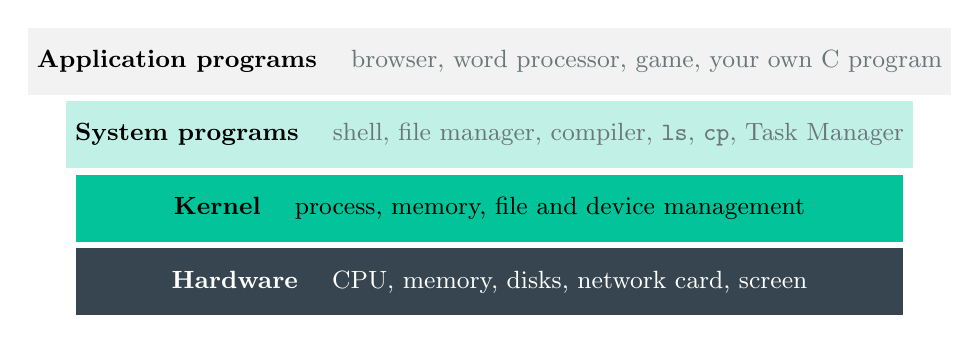
\begin{tikzpicture}[layer/.style={rectangle,minimum width=10.5cm,minimum height=0.85cm,align=center,font=\small}]
\node[layer,fill=light] (a) {\textbf{Application programs} \quad {\color{muted}browser, word processor, game, your own C program}};
\node[layer,fill=mint!25,below=2pt of a] (s) {\textbf{System programs} \quad {\color{muted}shell, file manager, compiler, \texttt{ls}, \texttt{cp}, Task Manager}};
\node[layer,fill=mint,below=2pt of s] (k) {\textbf{Kernel} \quad process, memory, file and device management};
\node[layer,fill=charcoal,text=white,below=2pt of k] (h) {\textbf{Hardware} \quad {\color{white!75}CPU, memory, disks, network card, screen}};
\end{tikzpicture}
\caption{Software layers on a typical computer.}
\end{figure}

\begin{itemize}
  \item The \textbf{kernel} is always in memory, runs in a privileged CPU mode (Section~\ref{sec:dualmode}) and talks directly to the hardware.
  \item \textbf{System programs} ship with the OS but run as ordinary programs. They make the system usable.
  \item \textbf{Application programs} are everything you install to do your actual work.
\end{itemize}

Strictly speaking, ``Linux'' is only a kernel. A \emph{Linux distribution} such as Ubuntu or Fedora adds thousands of system programs, most of them from the GNU Project.

\begin{histnote}[Is the web browser part of the OS?]
In 1998 the United States government sued Microsoft, partly over its claim that Internet Explorer was an integral part of Windows. The courts found that Microsoft had illegally maintained its monopoly, and the question ``what belongs to the OS?'' became a legal question as well as a technical one. A useful rule of thumb: the kernel is certainly the OS; beyond the kernel, ``the OS'' is whatever the vendor ships as the standard system.
\end{histnote}

% =====================================================================
\section{Design Goals of an Operating System}

William Stallings summarises the objectives of an operating system in three words.

\begin{enumerate}[leftmargin=1.4em]
  \item \textbf{Convenience.} The OS makes the computer easier to use and to program: files, windows, a shell, simple system calls. Users should not need to know the hardware.
  \item \textbf{Efficiency.} The OS uses the hardware well: the CPU busy with useful work, memory full of useful data, devices working in parallel. The OS itself should have low \term{overhead}, i.e.\ consume few resources of its own.
  \item \textbf{Ability to evolve.} New hardware (SSDs, GPUs, 5G modems) and new services must be addable without breaking existing programs. This goal, more than any other, drives the choice of OS \emph{structure} (Section~\ref{sec:structures}).
\end{enumerate}

\subsection{The goals conflict}

The three goals pull in different directions, and different kinds of computers weight them differently.

\begin{center}
\renewcommand{\arraystretch}{1.3}
\begin{tabularx}{\linewidth}{>{\raggedright\arraybackslash}p{3.3cm} >{\raggedright\arraybackslash}p{3.2cm} >{\raggedright\arraybackslash}X}
\toprule
\textbf{Kind of system} & \textbf{Main priority} & \textbf{Why} \\
\midrule
Personal computer & Convenience & One user who wants things to ``just work''; the CPU is idle most of the time anyway. \\
Server / cloud & Efficiency & Thousands of users; 1\% more throughput can mean hundreds of fewer machines. \\
Smartphone & Efficiency (energy) & Battery life: the OS aggressively puts apps and the CPU to sleep. \\
Embedded / IoT & Efficiency (size, cost) & A washing-machine controller may have a few kilobytes of memory; there may be no OS at all. \\
Real-time (brakes, drones) & Predictability & An answer that arrives late is a wrong answer: deadlines must always be met. \\
\bottomrule
\end{tabularx}
\end{center}

\begin{example}[Convenience versus efficiency]
A program must read $10^{6}$ numbers from a file. Suppose each system call (a request to the kernel, Section~\ref{sec:syscall}) costs $t_{s} \approx 0.1\ \mu\text{s}$ of pure overhead.
\begin{itemize}
  \item \emph{Convenient:} ask the OS for one number at a time: $10^{6}$ calls, overhead $10^{6} \times 0.1\ \mu\text{s} = 0.1\ \text{s} = 100\ \text{ms}$.
  \item \emph{Efficient:} ask for blocks of $4096$ bytes, about $10^{3}$ numbers each: $10^{3}$ calls, overhead $10^{3} \times 0.1\ \mu\text{s} = 0.1\ \text{ms}$.
\end{itemize}
The efficient version has $1000$ times less overhead. The C standard library gives you both: you call \cmd{fgetc()} one character at a time, but the library reads large blocks behind the scenes. This technique is called \term{buffering}.
\end{example}

% =====================================================================
\section{Components of a Computer System}

A computer system can be divided into four components.

\begin{figure}[H]
\centering
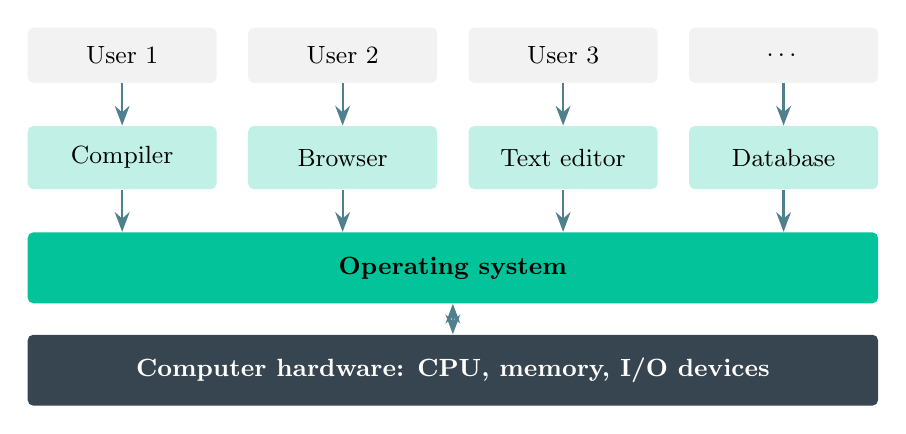
\begin{tikzpicture}[
  u/.style={rectangle,rounded corners=2pt,minimum width=2.4cm,minimum height=0.7cm,font=\small,fill=light},
  a/.style={rectangle,rounded corners=2pt,minimum width=2.4cm,minimum height=0.8cm,font=\small,fill=mint!25},
  big/.style={rectangle,rounded corners=2pt,minimum width=10.8cm,minimum height=0.9cm,font=\small\bfseries},
  arr/.style={-{Stealth[length=2.5mm]},color=slate,thick}]
\foreach \i/\t in {0/User 1,1/User 2,2/User 3,3/\dots} {
  \node[u] (u\i) at (\i*2.8,0) {\t};
  \node[a] (a\i) at (\i*2.8,-1.3) {};
  \draw[arr] (u\i) -- (a\i);
}
\node at (a0) {\small Compiler}; \node at (a1) {\small Browser}; \node at (a2) {\small Text editor}; \node at (a3) {\small Database};
\node[big,fill=mint] (os) at (4.2,-2.7) {Operating system};
\node[big,fill=charcoal,text=white] (hw) at (4.2,-4.0) {Computer hardware: CPU, memory, I/O devices};
\foreach \i in {0,1,2,3} \draw[arr] (a\i) -- (a\i |- os.north);
\draw[arr,{Stealth[length=2.5mm]}-{Stealth[length=2.5mm]}] (os) -- (hw);
\end{tikzpicture}
\caption{The four components of a computer system.}
\end{figure}

\begin{itemize}
  \item \textbf{Hardware} provides the basic computing resources: CPU, memory, input/output (I/O) devices.
  \item \textbf{Application programs} use these resources to solve the users' problems.
  \item \textbf{Users} are people, but also other machines and programs (e.g.\ a web server's ``users'' are other computers).
  \item \textbf{The operating system} controls the hardware and coordinates its use among the applications and users.
\end{itemize}

\subsection{Hardware organisation}

A modern computer has one or more CPUs and several \term{device controllers}, all connected by a common \term{bus} to shared main memory.

\begin{figure}[H]
\centering
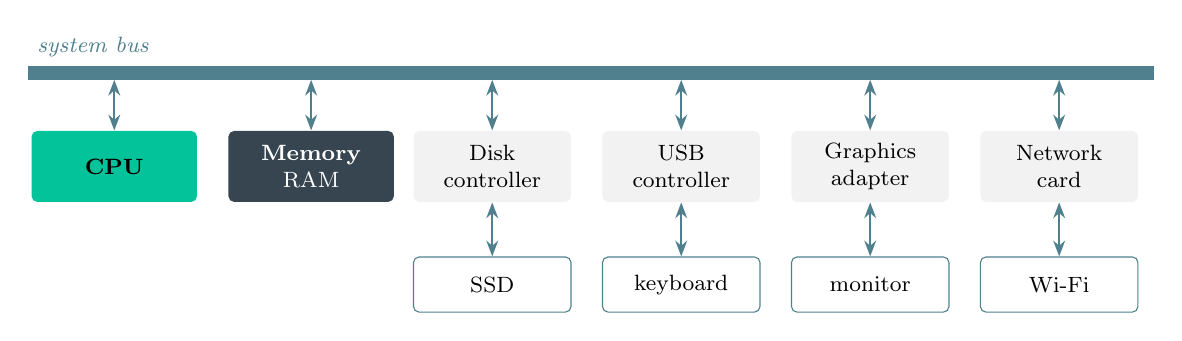
\begin{tikzpicture}[
  b/.style={rectangle,rounded corners=2pt,minimum width=2.1cm,minimum height=0.9cm,align=center,font=\footnotesize},
  arr/.style={{Stealth[length=2mm]}-{Stealth[length=2mm]},color=slate,thick}]
\fill[slate] (-0.3,0) rectangle (14.0,0.18);
\node[font=\footnotesize\itshape,text=slate,anchor=west] at (-0.3,0.42) {system bus};
\node[b,fill=mint] (cpu) at (0.8,-1.1) {\textbf{CPU}};
\node[b,fill=charcoal,text=white] (mem) at (3.3,-1.1) {\textbf{Memory}\\RAM};
\foreach \x/\t/\d in {6.0/Disk\\controller/SSD, 8.4/USB\\controller/keyboard, 10.8/Graphics\\adapter/monitor, 13.2/Network\\card/Wi-Fi} {
  \node[b,fill=light,minimum width=2.0cm] (c) at (\x-0.4,-1.1) {\t};
  \node[b,draw=slate,minimum width=2.0cm,minimum height=0.7cm] (dv) at (\x-0.4,-2.6) {\d};
  \draw[arr] (\x-0.4,0) -- (c.north);
  \draw[arr] (c.south) -- (dv.north);
}
\draw[arr] (0.8,0) -- (cpu.north);
\draw[arr] (3.3,0) -- (mem.north);
\end{tikzpicture}
\caption{CPU, memory and device controllers share the system bus.}
\end{figure}

Each device controller has a small local buffer and works \emph{in parallel} with the CPU. For each controller, the OS contains a \term{device driver}: a piece of software that understands the controller's commands and offers the rest of the OS a uniform interface.

\subsection{Interrupts}

How does the CPU find out that a device has finished its work? It could keep asking (``anything new?''), a technique called \term{polling}, but that wastes CPU time. Instead, the device \emph{tells} the CPU by raising an \term{interrupt}:

\begin{enumerate}[leftmargin=1.4em]
  \item The device controller finishes an operation (e.g.\ the data from the disk is now in its buffer).
  \item It sends a signal on an interrupt line to the CPU.
  \item The CPU saves the state of the program it was running and jumps to the \term{interrupt handler} whose address is stored in the \term{interrupt vector}, a table indexed by device number.
  \item The handler (part of the device driver, inside the OS) processes the event.
  \item The saved state is restored and the interrupted program continues as if nothing had happened.
\end{enumerate}

Modern operating systems are \textbf{interrupt-driven}: if no program wants to run and no device needs attention, the OS simply waits. Every key press, mouse movement, network packet and finished disk read arrives as an interrupt, often thousands per second.

\begin{example}[Why not just poll?]
A keyboard produces at most about $10$ key presses per second. Suppose checking the keyboard once takes $t_{\text{check}} = 1\ \mu\text{s}$ and, to feel responsive, we poll it $f = 1000$ times per second. The fraction of CPU time spent polling is
\[
f \cdot t_{\text{check}} = 1000\ \text{s}^{-1} \times 10^{-6}\ \text{s} = 10^{-3} = 0.1\%.
\]
That sounds small, but $99\%$ of those checks find nothing, and a computer has dozens of devices. With interrupts, the CPU spends time on the keyboard only when a key is actually pressed, about $10$ times per second.
\end{example}

\subsection{The storage hierarchy}

Storage comes in many types, which differ in speed, size, cost and \emph{volatility} (whether the content survives power-off).

\begin{center}
\renewcommand{\arraystretch}{1.3}
\begin{tabular}{@{}llll@{}}
\toprule
\textbf{Level} & \textbf{Typical size} & \textbf{Access time} & \textbf{If a register access took 1 s\dots} \\
\midrule
CPU registers & $< 1$ KB & $\approx 0.3$ ns & 1 second \\
Cache (L1--L3) & a few MB & $1$--$40$ ns & 3 seconds to 2 minutes \\
Main memory (RAM) & $8$--$64$ GB & $\approx 100$ ns & $\approx 5$ minutes \\
Solid-state drive (SSD) & $0.5$--$4$ TB & $\approx 50\ \mu$s & $\approx 2$ days \\
Hard disk drive (HDD) & $1$--$20$ TB & $\approx 5$ ms & $\approx 6$ months \\
\bottomrule
\end{tabular}
\end{center}

The last column multiplies every access time by the same factor $1/(0.3\ \text{ns}) \approx 3.3\times10^{9}$; for example, for a hard disk $5\ \text{ms} \times 3.3\times10^{9} \approx 1.7\times10^{7}\ \text{s} \approx 190$ days. Registers, cache and RAM are \textbf{volatile}; SSDs and disks are \textbf{non-volatile}. Much of the OS's work consists of moving data between levels so that the data a program needs is in fast storage when it needs it. We return to this in Weeks~6 and~7.

\subsection{Dual-mode operation}
\label{sec:dualmode}

If any program could do anything, one buggy or malicious program could destroy all the others. Protection therefore needs \emph{hardware} support. The CPU has a \term{mode bit}:

\begin{itemize}
  \item \textbf{Kernel mode} (also: supervisor, system or privileged mode; mode bit $=0$): every instruction is allowed. Only the OS kernel runs in this mode.
  \item \textbf{User mode} (mode bit $=1$): \term{privileged instructions}, such as direct I/O, changing memory protection or halting the CPU, are forbidden.
\end{itemize}

If a user program tries a privileged instruction, the hardware does not execute it; instead it \emph{traps} to the OS, which usually terminates the program. When a program needs a privileged service, it makes a \term{system call}: a special instruction that switches to kernel mode and jumps to a fixed entry point in the kernel. When the kernel is done, it switches back to user mode and returns.

\begin{figure}[H]
\centering
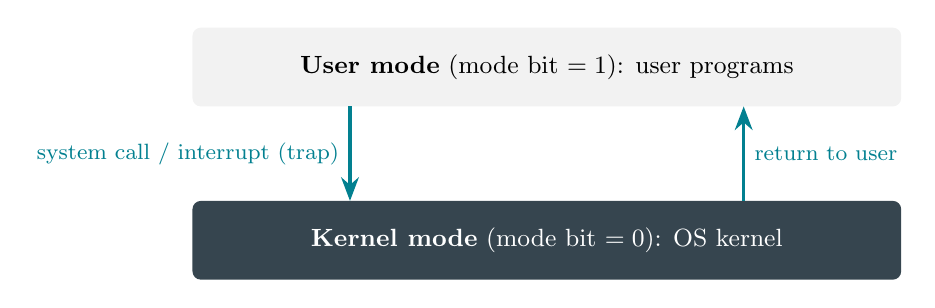
\begin{tikzpicture}[
  m/.style={rectangle,rounded corners=3pt,minimum width=9cm,minimum height=1.0cm,align=center,font=\small},
  arr/.style={-{Stealth[length=3mm]},very thick,color=mintdeep}]
\node[m,fill=light] (u) at (0,2.2) {\textbf{User mode} (mode bit $= 1$): user programs};
\node[m,fill=charcoal,text=white] (k) at (0,0) {\textbf{Kernel mode} (mode bit $= 0$): OS kernel};
\draw[arr] (-2.5,1.7) -- node[left,font=\footnotesize,text=mintdeep]{system call / interrupt (trap)} (-2.5,0.5);
\draw[arr] (2.5,0.5) -- node[right,font=\footnotesize,text=mintdeep]{return to user} (2.5,1.7);
\end{tikzpicture}
\caption{Switching between user mode and kernel mode.}
\end{figure}

On x86 processors the modes are called \emph{rings}, numbered $0$ (most privileged) to $3$; Linux and Windows use only ring~0 (kernel) and ring~3 (user). The MS-DOS story in Section~\ref{sec:simple} shows what happens without this protection.

% =====================================================================
\section{Hands-on: Watching a Program Call the Kernel}
\label{sec:syscall}

The programs in this section are in the \texttt{code/} folder next to these notes. They are written in C for Linux. You can compile them on the lab computers, in WSL (Windows Subsystem for Linux), or in an online C compiler. You are \emph{not} expected to write C in this course; read the comments and focus on what the program does.

\subsection{Example 1: library call versus system call}

\lstinputlisting[caption={}]{../code/hello_syscall.c}

\cmd{printf()} is a \emph{library function}: it runs entirely in user mode and formats the text. To actually put characters on the screen it must ask the kernel, using the \cmd{write()} system call. The program \cmd{strace} shows every system call another program makes:

\begin{lstlisting}[style=term]
$ gcc hello_syscall.c -o hello_syscall
$ strace ./hello_syscall
...
write(1, "Hello from printf!\n", 19)  = 19
write(1, "Hello from write()!\n", 20) = 20
exit_group(0)                         = ?
\end{lstlisting}

Both lines end up as the same \cmd{write} system call. The numbers are: file descriptor $1$ (standard output, the screen), the bytes to write, their count, and, after the \texttt{=}, the value returned by the kernel (the number of bytes actually written).

Even a simple command makes many system calls. On our test machine \cmd{strace -c ls /} reported $76$ system calls, most of them to open, read, map into memory and close files.

\subsection{Example 2: how expensive is a system call?}

\lstinputlisting[caption={}]{../code/syscall_cost.c}

Sample output on our test machine (a Linux virtual machine):

\begin{lstlisting}[style=term]
$ gcc -O2 syscall_cost.c -o syscall_cost
$ ./syscall_cost
ordinary function call :    1.5 ns
system call (getpid)   :  116.1 ns
system call is about 76 times slower
\end{lstlisting}

Your numbers will differ: on a typical PC, a minimal system call costs roughly $50$--$200$ ns, while a function call costs about $1$--$2$ ns. The ratio is the lesson: crossing the boundary between user mode and kernel mode is \emph{expensive}, because the CPU must save registers, switch modes, check the request and switch back. Keep this in mind for Section~\ref{sec:micro}.

\begin{example}[How much overhead is that?]
With $t_{\text{func}} = 1.5$ ns and $t_{\text{sys}} = 116$ ns, making $N = 10^{6}$ system calls instead of function calls adds
\[
N\,(t_{\text{sys}} - t_{\text{func}}) = 10^{6} \times (116 - 1.5)\ \text{ns} \approx 1.1\times10^{8}\ \text{ns} \approx 0.11\ \text{s}.
\]
\end{example}

% =====================================================================
\section{Operating-System Structures}
\label{sec:structures}

A general-purpose OS is a very large program; the Linux kernel alone has over $30$ million lines of source code, most of it device drivers. How such a program is organised has a large effect on its speed, reliability and ability to evolve. We look at six approaches.

\subsection{Simple structure: MS-DOS}
\label{sec:simple}

MS-DOS (1981) was written to provide the most functionality in the least space on the original IBM PC. It was not divided into carefully separated modules.

\begin{figure}[H]
\centering
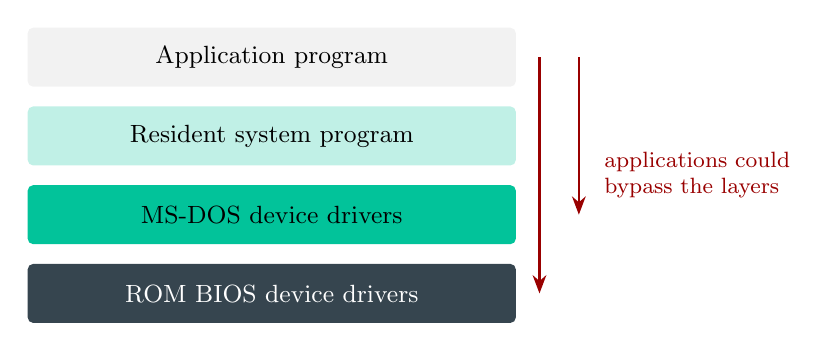
\begin{tikzpicture}[l/.style={rectangle,rounded corners=2pt,minimum width=6.2cm,minimum height=0.75cm,font=\small}]
\node[l,fill=light] (a) at (0,3.0) {Application program};
\node[l,fill=mint!25] (r) at (0,2.0) {Resident system program};
\node[l,fill=mint] (d) at (0,1.0) {MS-DOS device drivers};
\node[l,fill=charcoal,text=white] (b) at (0,0) {ROM BIOS device drivers};
\draw[-{Stealth},thick,red!60!black] (3.4,3.0) -- (3.4,0.0);
\draw[-{Stealth},thick,red!60!black] (3.9,3.0) -- (3.9,1.0);
\node[font=\footnotesize,text=red!60!black,align=left,anchor=west] at (4.1,1.5) {applications could\\bypass the layers};
\end{tikzpicture}
\caption{MS-DOS layer structure: programs could reach the hardware directly.}
\end{figure}

Application programs could bypass the OS and write directly to the display or the disk. The Intel 8088 processor of the IBM PC had \emph{no} dual mode, so the OS had no way to stop them. As a result, one buggy program could crash the entire system. \textbf{Lesson:} protection requires both hardware support and an OS that uses it.

\subsection{Monolithic kernel: UNIX and Linux}

In a \term{monolithic} kernel, all OS services (process scheduling, memory management, file systems, networking, device drivers) form one large program that runs in kernel mode, in a single address space.

\begin{figure}[H]
\centering
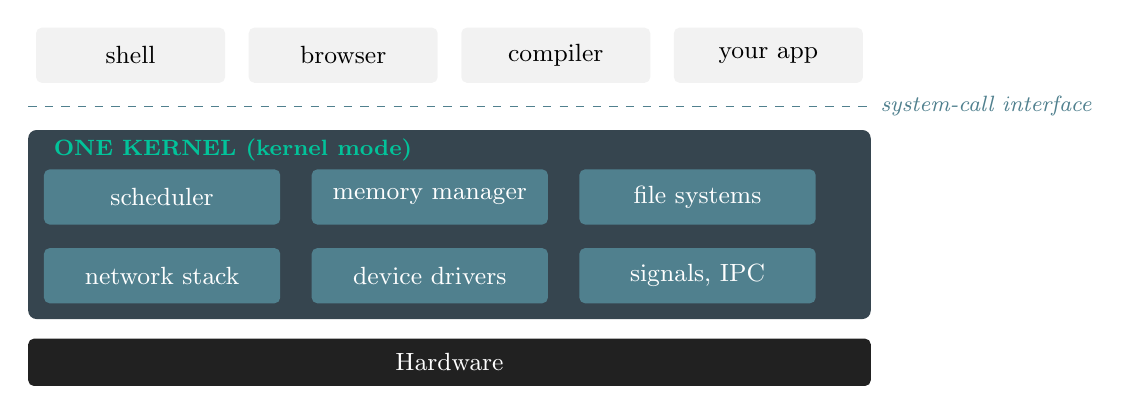
\begin{tikzpicture}[s/.style={rectangle,rounded corners=2pt,minimum width=2.4cm,minimum height=0.7cm,font=\small}]
\foreach \i/\t in {0/shell,1/browser,2/compiler,3/your app} \node[s,fill=light] at (\i*2.7,2.4) {\t};
\draw[dashed,slate] (-1.3,1.75) -- (9.4,1.75) node[right,font=\footnotesize\itshape,text=slate] {system-call interface};
\fill[charcoal,rounded corners=3pt] (-1.3,-0.95) rectangle (9.4,1.45);
\node[font=\footnotesize\bfseries,text=mint,anchor=west] at (-1.1,1.2) {ONE KERNEL (kernel mode)};
\foreach \i/\t in {0/scheduler,1/memory manager,2/file systems} \node[s,fill=slate,text=white,minimum width=3.0cm] at (\i*3.4+0.4,0.6) {\t};
\foreach \i/\t in {0/network stack,1/device drivers,2/{signals, IPC}} \node[s,fill=slate,text=white,minimum width=3.0cm] at (\i*3.4+0.4,-0.4) {\t};
\node[rectangle,rounded corners=2pt,minimum width=10.7cm,minimum height=0.6cm,fill=dark,text=white,font=\small] at (4.05,-1.5) {Hardware};
\end{tikzpicture}
\caption{A monolithic kernel.}
\end{figure}

\begin{itemize}
  \item[\textcolor{mintdeep}{$+$}] \textbf{Fast:} kernel components call each other directly, like ordinary function calls; a system call needs only two mode switches.
  \item[\textcolor{red!60!black}{$-$}] \textbf{Hard to maintain:} millions of lines in one program.
  \item[\textcolor{red!60!black}{$-$}] \textbf{Fragile:} a bug in any part, typically a driver, can crash the whole kernel (a \emph{kernel panic} on Linux, a ``blue screen'' on Windows).
\end{itemize}
Examples: the original UNIX (1970s), Linux, traditional BSD.

\subsection{Layered approach}

The OS is divided into layers. Layer $0$ is the hardware; the highest layer is the user interface. Each layer may use only the services of the layers below it.

\begin{figure}[H]
\centering
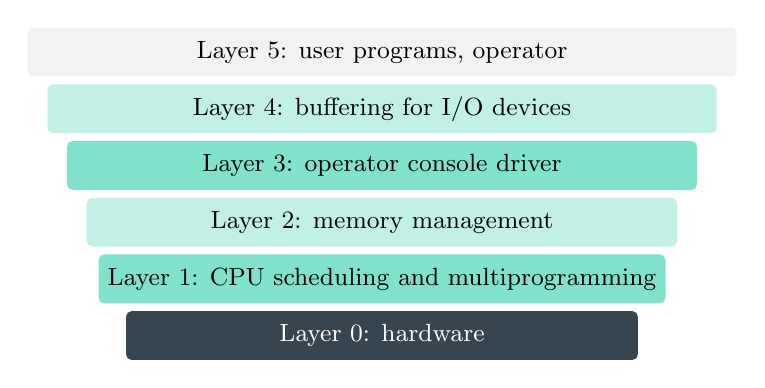
\begin{tikzpicture}
\foreach \i/\t/\c in {0/{Layer 5: user programs, operator}/light, 1/{Layer 4: buffering for I/O devices}/mint!25, 2/{Layer 3: operator console driver}/mint!50, 3/{Layer 2: memory management}/mint!25, 4/{Layer 1: CPU scheduling and multiprogramming}/mint!50, 5/{Layer 0: hardware}/charcoal} {
  \pgfmathsetmacro{\w}{9-0.5*\i}
  \node[rectangle,rounded corners=2pt,minimum width=\w cm,minimum height=0.62cm,fill=\c,font=\small] at (0,-0.72*\i) {\ifnum\i=5 \color{white}\fi\t};
}
\end{tikzpicture}
\caption{A layered OS, loosely based on Dijkstra's THE system (1968).}
\end{figure}

\begin{itemize}
  \item[\textcolor{mintdeep}{$+$}] Easy to construct and debug: test layer 1 first, then layer 2 on top of it, and so on.
  \item[\textcolor{red!60!black}{$-$}] It is hard to decide the order of the layers. Memory management needs the scheduler (to wait for a disk), but the scheduler needs memory (for its tables). Which goes first?
  \item[\textcolor{red!60!black}{$-$}] Each request passes through many layers, each adding overhead.
\end{itemize}

Pure layering is rare in general-purpose systems today, but the idea survives inside every OS; the network stack, for example, is strictly layered.

\subsection{Microkernel}
\label{sec:micro}

The \term{microkernel} approach removes everything non-essential from the kernel and runs it as ordinary user-mode programs called \emph{servers}. The microkernel itself provides only minimal process and memory management and, above all, \term{message passing} between programs.

\begin{figure}[H]
\centering
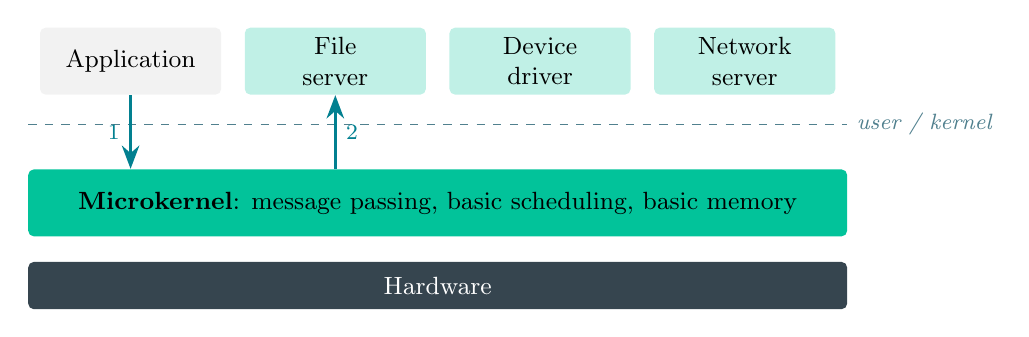
\begin{tikzpicture}[s/.style={rectangle,rounded corners=2pt,minimum width=2.3cm,minimum height=0.85cm,font=\small,align=center}]
\node[s,fill=light] (app) at (0,2.4) {Application};
\node[s,fill=mint!25] (fs) at (2.6,2.4) {File\\server};
\node[s,fill=mint!25] at (5.2,2.4) {Device\\driver};
\node[s,fill=mint!25] at (7.8,2.4) {Network\\server};
\draw[dashed,slate] (-1.3,1.6) -- (9.1,1.6) node[right,font=\footnotesize\itshape,text=slate] {user / kernel};
\node[rectangle,rounded corners=2pt,minimum width=10.4cm,minimum height=0.85cm,fill=mint,font=\small] (mk) at (3.9,0.6) {\textbf{Microkernel}: message passing, basic scheduling, basic memory};
\node[rectangle,rounded corners=2pt,minimum width=10.4cm,minimum height=0.6cm,fill=charcoal,text=white,font=\small] at (3.9,-0.45) {Hardware};
\draw[-{Stealth},very thick,mintdeep] (app.south) -- node[left,font=\footnotesize]{1} (app.south |- mk.north);
\draw[-{Stealth},very thick,mintdeep] (fs.south |- mk.north) -- node[right,font=\footnotesize]{2} (fs.south);
\end{tikzpicture}
\caption{In a microkernel, an application's request to the file server travels as a message through the kernel.}
\end{figure}

\begin{itemize}
  \item[\textcolor{mintdeep}{$+$}] \textbf{Reliable:} a crashed driver is just a crashed user program; the system can restart it.
  \item[\textcolor{mintdeep}{$+$}] \textbf{Secure and extensible:} new services are new user programs; the small kernel is easier to check. The seL4 microkernel has even been \emph{mathematically proven} correct.
  \item[\textcolor{red!60!black}{$-$}] \textbf{Slower:} every service request needs extra messages and mode switches.
\end{itemize}
Examples: Mach (Carnegie Mellon, 1980s), MINIX~3, QNX (used in cars and medical devices), L4 and seL4.

\begin{example}[The price of a microkernel]
Count the mode switches for one file read.
\begin{itemize}
  \item Monolithic: application $\to$ kernel $\to$ application: $2$ switches.
  \item Microkernel: application $\to$ kernel $\to$ file server $\to$ kernel $\to$ application: $4$ switches, plus $2$ message copies.
\end{itemize}
Take illustrative values: a mode switch costs $t_{s} = 0.1\ \mu\text{s}$, a message copy $t_{c} = 0.15\ \mu\text{s}$, and the useful work $t_{w} = 1\ \mu\text{s}$. Then
\[
T_{\text{mono}} = 2t_{s} + t_{w} = 0.2 + 1.0 = 1.2\ \mu\text{s},
\qquad
T_{\mu} = 4t_{s} + 2t_{c} + t_{w} = 0.4 + 0.3 + 1.0 = 1.7\ \mu\text{s},
\]
so the microkernel is $T_{\mu}/T_{\text{mono}} \approx 1.42$ times, i.e.\ about $42\%$, slower for this operation. For long operations (large $t_{w}$) the ratio approaches $1$ and the overhead hardly matters:
\[
\lim_{t_{w}\to\infty} \frac{4t_{s} + 2t_{c} + t_{w}}{2t_{s} + t_{w}} = 1 .
\]
\end{example}

\subsection{Modular kernel: loadable kernel modules}

Most modern systems use a \term{modular} design: a core kernel plus \term{loadable kernel modules} that can be added or removed while the system is running. When you plug in a USB device, Linux can load the right driver module automatically.

\begin{itemize}
  \item[\textcolor{mintdeep}{$+$}] Like a monolithic kernel, modules run in kernel mode, so calls between them are fast.
  \item[\textcolor{mintdeep}{$+$}] Like a microkernel, the system is flexible: only the modules that are needed are loaded.
  \item[\textcolor{red!60!black}{$-$}] A buggy module still runs in kernel mode and can still crash the system.
\end{itemize}
Examples: Linux, Solaris, the modern BSDs.

\paragraph{Example 3: a minimal kernel module.} The listing below is the standard ``hello world'' Linux kernel module. It has no \cmd{main()}; instead, the kernel calls \cmd{hello\_init()} when the module is loaded and \cmd{hello\_exit()} when it is removed. Its messages go to the kernel log, not to the screen.

\lstinputlisting[caption={}]{../code/hello_module.c}

\begin{lstlisting}[style=term]
$ make                          # needs the kernel-headers package
$ sudo insmod hello_module.ko   # load
$ lsmod | grep hello            # is it there?
$ sudo dmesg | tail -1          # read the kernel log
hello_module: loaded into the kernel
$ sudo rmmod hello_module       # unload
\end{lstlisting}

\begin{tryit}[Safety first]
Code in a kernel module runs in kernel mode: a mistake can freeze the whole computer. Only try Example~3 inside a virtual machine. It is shown here so that you can \emph{see} what ``loadable module'' means; you will not need to write one.
\end{tryit}

\subsection{Hybrid systems}

Real operating systems rarely follow one pure design.

\begin{itemize}
  \item \textbf{Windows (NT family)} was designed with microkernel ideas (separate subsystems), but for speed most services, including graphics, run in kernel mode. Drivers are loadable, like modules.
  \item \textbf{macOS and iOS} use the \emph{XNU} kernel, which combines the Mach microkernel with parts of BSD UNIX, compiled into a single kernel, plus loadable kernel extensions.
  \item \textbf{Android} uses a modified Linux kernel (monolithic plus modules), with a hardware abstraction layer, native libraries and the Android runtime for apps on top.
\end{itemize}

\begin{histnote}[The Tanenbaum--Torvalds debate (1992)]
In January 1992, Andrew Tanenbaum, author of the MINIX microkernel, posted a message titled ``LINUX is obsolete'', arguing that a monolithic kernel was ``a giant step back into the 1970s''. Linus Torvalds replied that Linux worked and was fast. More than thirty years later, both designs are in daily use: Linux on servers and phones, microkernels in cars, aircraft and other safety-critical devices.
\end{histnote}

\subsection{Comparison}

\begin{center}
\renewcommand{\arraystretch}{1.3}
\begin{tabular}{@{}lllll@{}}
\toprule
\textbf{Structure} & \textbf{In kernel mode} & \textbf{Speed} & \textbf{Reliability} & \textbf{Example} \\
\midrule
Simple & everything (no protection) & high & very low & MS-DOS \\
Monolithic & all OS services & high & medium & UNIX, Linux \\
Layered & all layers & low & high & THE (1968) \\
Microkernel & only the tiny kernel & lower & high & MINIX 3, QNX, seL4 \\
Modular & core + loaded modules & high & medium & Linux, Solaris \\
Hybrid & varies & high & medium--high & Windows, macOS, Android \\
\bottomrule
\end{tabular}
\end{center}

The recurring trade-off: every boundary you add (a layer, a message, a mode switch) buys reliability and costs speed.

% =====================================================================
\section{Summary}

\begin{keyidea}[Week 2 in six sentences]
\begin{enumerate}[leftmargin=1.4em]
  \item The OS manages the hardware and offers programs a simpler, safer machine; its always-resident core is the kernel.
  \item It can be seen top-down as an extended machine (abstraction) or bottom-up as a resource manager (time and space multiplexing).
  \item Its three design goals are convenience, efficiency and the ability to evolve, weighted differently on PCs, servers, phones and embedded systems.
  \item A computer system has four components: hardware, OS, application programs and users; devices signal the CPU with interrupts.
  \item Dual-mode operation protects the system; a system call switches to kernel mode and costs far more than a function call.
  \item OS structures (simple, monolithic, layered, microkernel, modular, hybrid) are different compromises between speed and reliability.
\end{enumerate}
\end{keyidea}

% =====================================================================
\Needspace{12\baselineskip}
\section{Glossary}

\begin{description}[leftmargin=0pt,style=nextline,itemsep=0.2em]
  \item[Abstraction] A simplified view that hides details, e.g.\ a \emph{file} instead of disk sectors.
  \item[Buffering] Collecting data into large blocks to reduce the number of expensive operations.
  \item[Device driver] OS code that controls one type of device controller.
  \item[Dual-mode operation] Hardware support for two CPU modes, user and kernel, selected by a mode bit.
  \item[Interrupt] A signal from hardware that makes the CPU stop, run an OS handler, and then resume.
  \item[Interrupt vector] A table of handler addresses, indexed by interrupt number.
  \item[Kernel] The part of the OS that is always in memory and runs in kernel mode.
  \item[Loadable kernel module] Code that can be added to or removed from a running kernel.
  \item[Microkernel] A minimal kernel; most OS services run as user-mode server programs that communicate by messages.
  \item[Monolithic kernel] A kernel in which all OS services run as one program in kernel mode.
  \item[Multiplexing] Sharing a resource in time (taking turns) or in space (dividing it).
  \item[Privileged instruction] An instruction that the CPU executes only in kernel mode.
  \item[System call] A request from a program to the kernel; it switches the CPU to kernel mode.
  \item[Trap] A software-generated interrupt, caused by a system call or an error.
\end{description}

% =====================================================================
\Needspace{20\baselineskip}
\section{Try It Yourself}

\begin{tryit}[Look inside your own operating system]
\textbf{Linux} (lab PCs, WSL, or a virtual machine):
\begin{lstlisting}[style=term]
$ uname -r          # which kernel version?
$ lsmod | head      # which modules are loaded?
$ strace -c ls      # count the system calls made by ls
\end{lstlisting}
\textbf{Windows:} run \cmd{winver} (Windows build) and \cmd{driverquery} (installed drivers) in a Command Prompt. In Task Manager $\to$ \emph{Performance} $\to$ CPU, right-click the graph and choose \emph{Show kernel times}.
\begin{enumerate}[leftmargin=1.4em]
  \item How many kernel modules are loaded on your machine?
  \item Which system call does \cmd{ls} use most often?
  \item Find a program that spends a lot of time in kernel mode. Why might that be?
\end{enumerate}
\end{tryit}

% =====================================================================
\section{Review Questions}

\subsection*{Conceptual}
\begin{enumerate}[leftmargin=1.6em]
  \item Give the three textbook definitions of an operating system. Which aspect does each emphasise?
  \item Explain the difference between the ``extended machine'' and ``resource manager'' views. Give an example of each.
  \item Give one example of time multiplexing and one of space multiplexing.
  \item What is the difference between the kernel and a system program? Is the shell part of the kernel?
  \item Name the three design goals of an OS. Which one matters most for (a) a smartphone, (b) a web server, (c) a car's brake controller?
  \item Describe, step by step, what happens when a disk controller raises an interrupt.
  \item Why must protection be supported by the hardware? What would happen on a CPU without dual mode?
  \item What is the difference between \cmd{printf()} and \cmd{write()}?
  \item Compare monolithic and microkernel designs: one advantage and one disadvantage of each.
  \item Why is a modular kernel described as ``the best of both worlds''? What is its remaining weakness?
\end{enumerate}

\subsection*{Numerical}
\begin{enumerate}[leftmargin=1.6em,resume]
  \item A system call costs $0.2\ \mu$s. A program reads a $1$~MB file (a) one byte at a time, (b) in blocks of $4096$ bytes. Compute the system-call overhead in each case. (Take $1\ \text{MB} = 2^{20}$ bytes.)
  \item A device is polled $500$ times per second; each check takes $2\ \mu$s. What fraction of the CPU is spent polling? How many CPU-seconds per day is that?
  \item Using the scale ``register access $=1$ s'', how long would an access to RAM ($80$ ns) and to an SSD ($100\ \mu$s) take? Take the register access time as $0.3$ ns.
  \item In the microkernel example, the useful work grows to $t_{w} = 10\ \mu$s. Compute the slow-down $T_{\mu}/T_{\text{mono}}$. What does this tell you?
\end{enumerate}

\subsection*{Answers to the numerical questions}
\begin{enumerate}[leftmargin=1.6em,start=11]
  \item (a) $2^{20}$ calls $\times\, 0.2\ \mu\text{s} \approx 0.21$ s. (b) $2^{20}/2^{12} = 256$ calls $\times\, 0.2\ \mu\text{s} \approx 51\ \mu\text{s}$, i.e.\ $4096$ times less.
  \item $500 \times 2\times10^{-6} = 10^{-3} = 0.1\%$. Per day: $0.001 \times 86\,400\ \text{s} \approx 86$ CPU-seconds.
  \item Scale factor $1/(0.3\ \text{ns}) \approx 3.33\times10^{9}$. RAM: $80\times10^{-9} \times 3.33\times10^{9} \approx 267$ s $\approx 4.4$ min. SSD: $10^{-4} \times 3.33\times10^{9} \approx 3.3\times10^{5}$ s $\approx 3.9$ days.
  \item $T_{\text{mono}} = 0.2 + 10 = 10.2\ \mu$s, $T_{\mu} = 0.4 + 0.3 + 10 = 10.7\ \mu$s; ratio $\approx 1.05$, only $5\%$ slower. The microkernel overhead matters for short, frequent operations, not for long ones.
\end{enumerate}

% =====================================================================
\section{Looking Ahead: Week 3}

\begin{itemize}
  \item The services an operating system provides to users and programs.
  \item System calls in detail: types, parameter passing, the system-call table.
  \item The process concept: a program in execution, and its memory layout.
  \item Process states: new, ready, running, waiting, terminated; the process control block.
\end{itemize}

\subsection*{Further reading (optional)}
\begin{itemize}
  \item A.\ Silberschatz, P.\,B.\ Galvin and G.\ Gagne, \emph{Operating System Concepts}, 10th ed., Wiley, Chapters~1--2.
  \item W.\ Stallings, \emph{Operating Systems: Internals and Design Principles}, 9th ed., Pearson, Chapter~2.
  \item A.\,S.\ Tanenbaum and H.\ Bos, \emph{Modern Operating Systems}, 4th ed., Pearson, Sections~1.1 and~1.7.
  \item R.\,H.\ and A.\,C.\ Arpaci-Dusseau, \emph{Operating Systems: Three Easy Pieces}, Chapter~6, ``Limited Direct Execution'': \url{https://pages.cs.wisc.edu/~remzi/OSTEP/cpu-mechanisms.pdf}
\end{itemize}

\end{document}
